\section{Power Gating and Adaptive-Precision Implementation}\label{strategy}

\subsection{Implementation of Power Gating}

The power gating can be implemented simply by adding PMOS-transistor switches between the functional blocks and the supply voltage \cite{keating_low_2007} as presented in Fig.~\ref{GATING}. 
When the switches are turned off, the corresponding blocks’ current paths will be cut off and thereby the energy is saved. 

It is obvious that for analog circuits, the more current is under control, the more effective the power gating can be. However, to avoid unacceptable IR drop, the total size of the switches may be large, 
and inverters should be inserted between the control signal and the switches’ gates for sufficient driving capability. 

Besides, the longer time the functional blocks can be power off, the better power scaling capacity can be obtained. And a continuous long time is preferred than separated short time for power gating because the blocks' metastability should also be taken into consideration.
As presented in Fig.~\ref{TIME}, separated short time for power gating will inevitably waste more
time for the blocks' shut down or recovery. 

As the collumn-parallel ADCs not only have large amounts of column-parallel currents that can be controlled, but also offer continuously and exponentially scalable power-off time thanks to the widely adopted SS conversion logic, applying power gating to this architecture will be highly promising.

\begin{figure}[htbp]
	\centerline{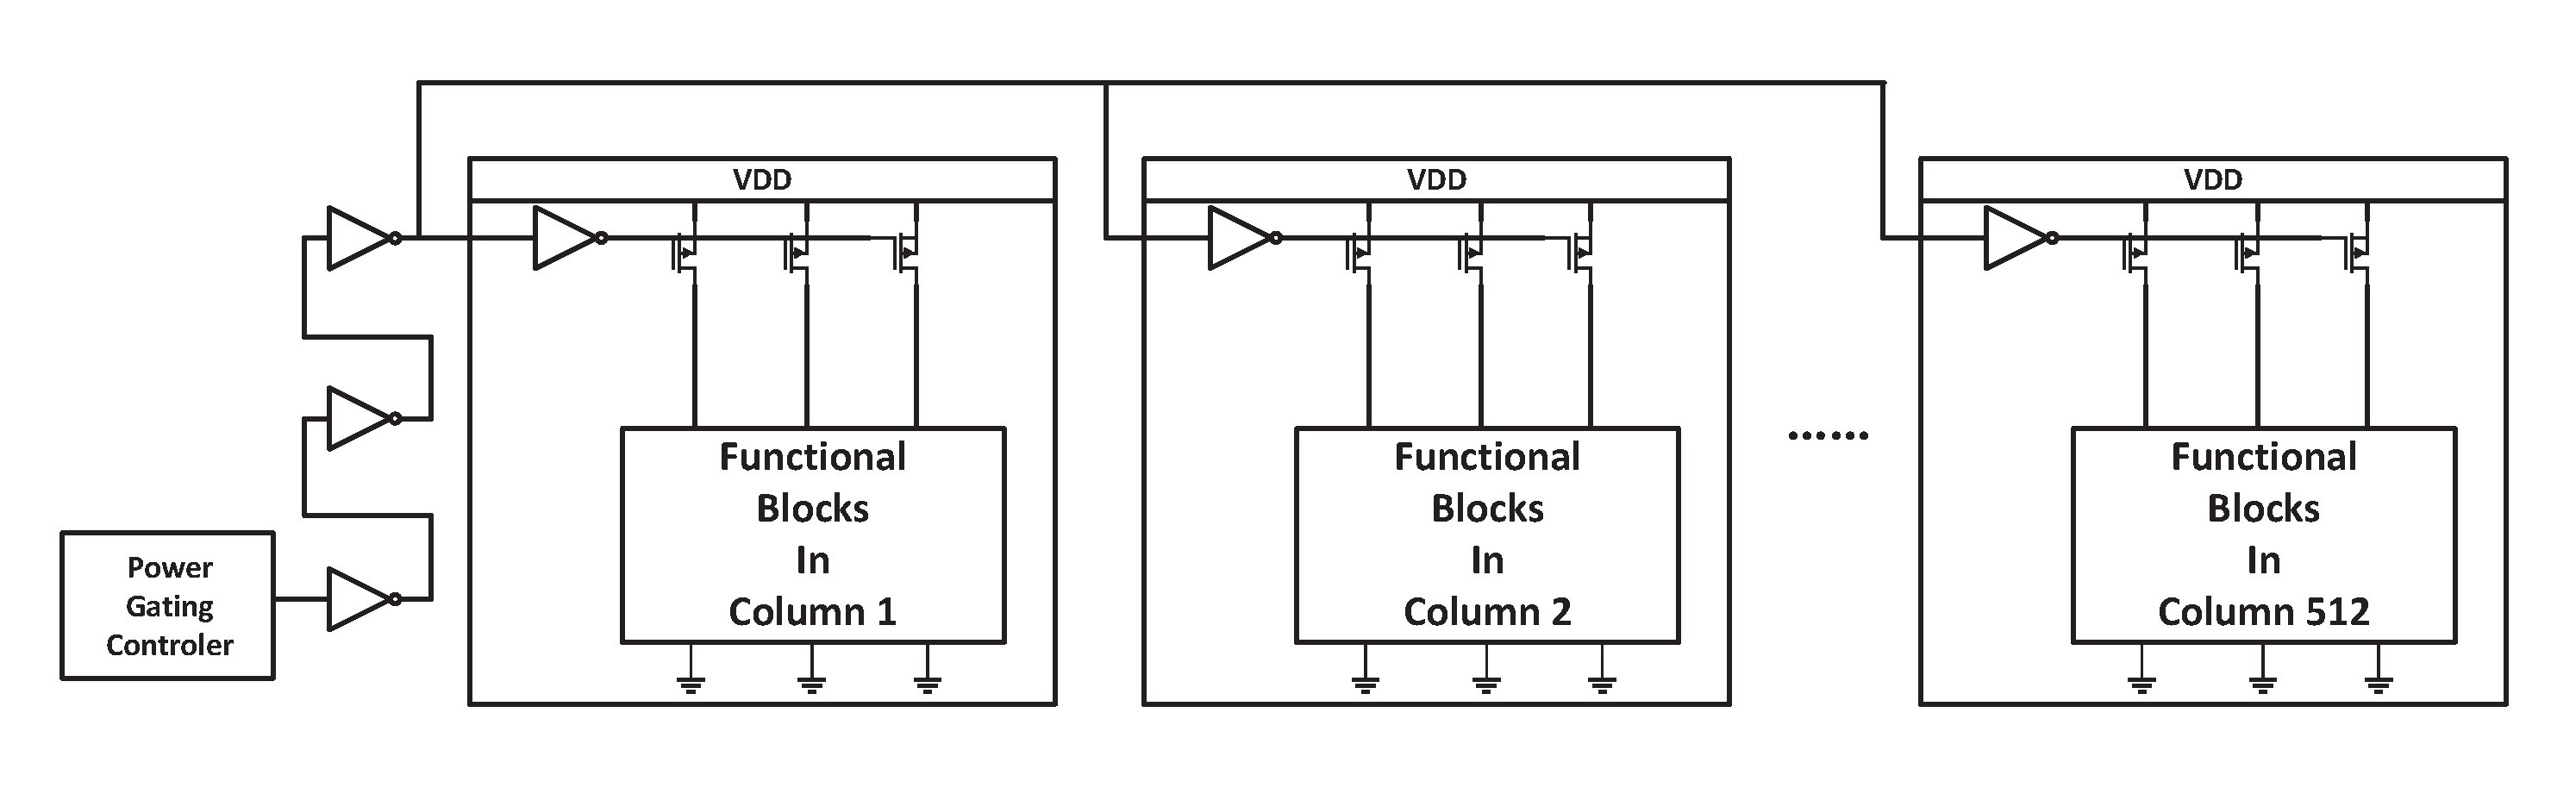
\includegraphics[width=3.5in]{./Figures/GATING.eps}}
	\caption{Implementation of Power Gating}
	\label{GATING}
\end{figure} 

\begin{figure}[htbp]
	\centerline{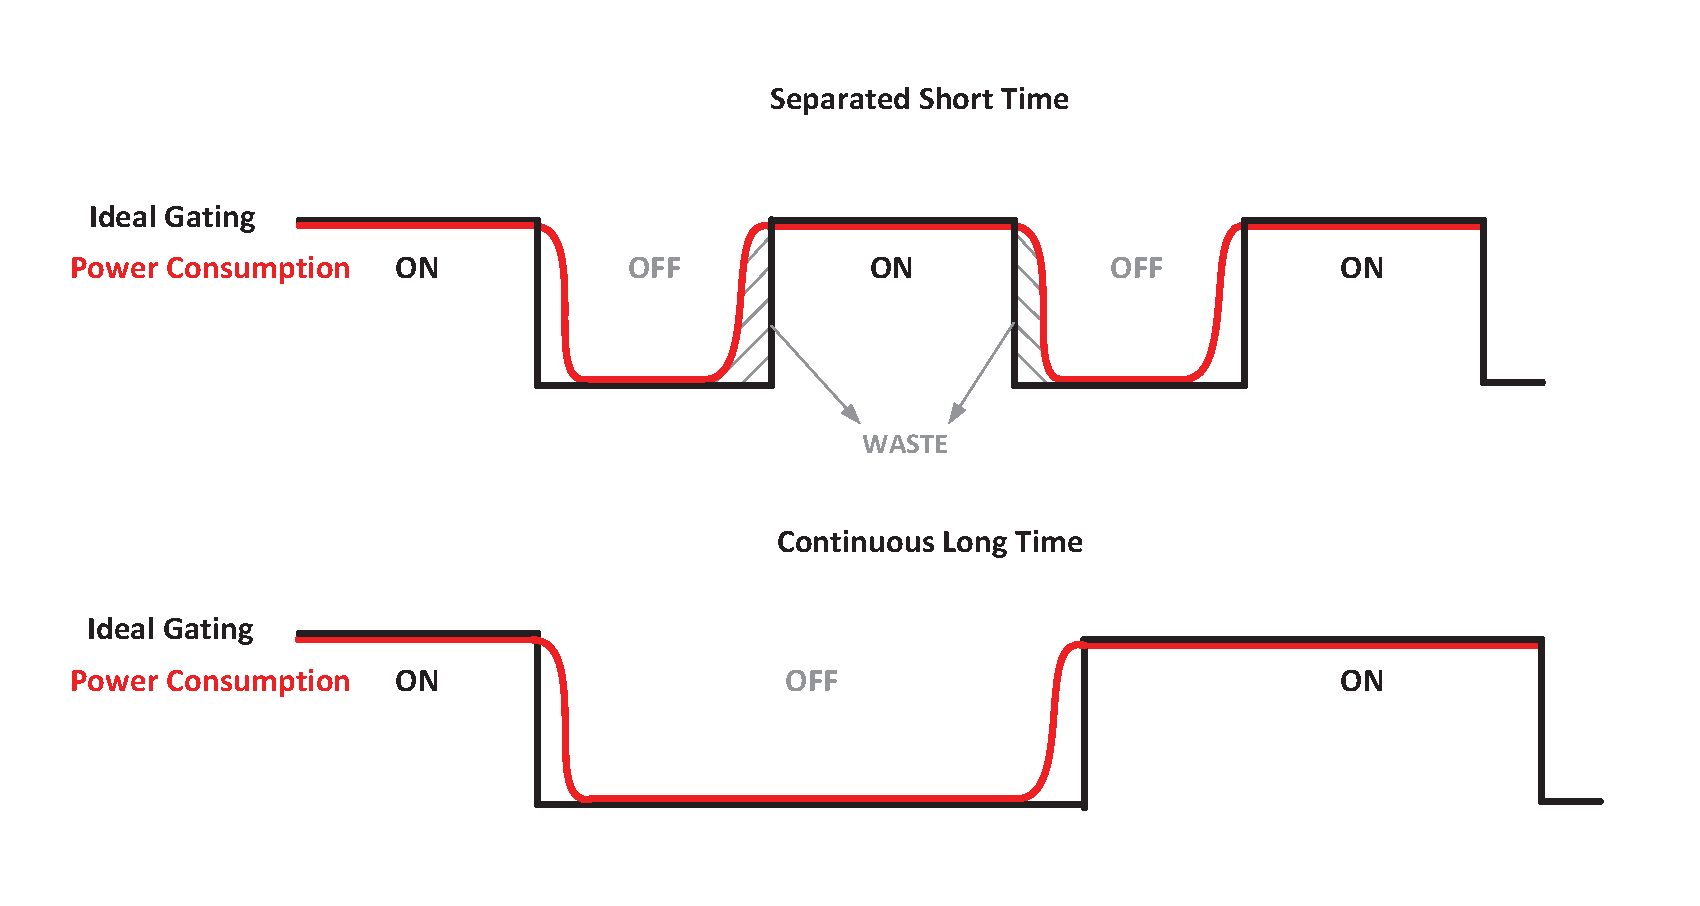
\includegraphics[width=3.5in]{./Figures/TIME.eps}}
	\caption{Continuous Long Time versus Separated Short Time for Power Gating.}
	\label{TIME}
\end{figure}  

\subsection{Adaptive-Precision Implementation for the SS ADCs}

As evaluated in Sect.~\ref{result}, the SS ADCs’ power consumption is mainly taken up by the column-parallel comparators, bias circuits, and the output buffer of the ramp generator. 
Considering that all bias circuits are settled down only once (tens of microseconds after the whole system's power up) and then other circuits can be settled down quickly by the distributed 
bias circuits, we just apply power gating to the amplifiers in the comparators and the output buffer in the ramp generator.

For low-precision conversion, the thermometer counter should have been extended to support switching the capacitors in CDAC 16 by 16 instead of one by one and thereby the ramp signal can reach $V_{refh}$ in 16 steps (for 4 bits) instead of in 256 steps (for 8 bits). 
After the 16 steps, the comparators and the output buffer can be power off for an extented period of time, leaving the related signals decrease gradually.
The related waveform are presented in Fig.~\ref{SS_pg}. 

To avoid the decreasing output of comparators causing extra unwanted latch for the low-precision conversion results, an NMOS switch and a PMOS switch are added to the two inverters fowllowing the comparator as presented in Fig.~\ref{MATE}. 
For high-precision conversion, the gating signal will be low-level and turn on the PMOS switch, thus the second inverter's output will be the same as the comparator's output, which is either low-level or high-level. 
For low-precision conversion, the NMOS switch is turned on by the high-level gating signal and the second inverter's input is connected to the ground. Therefore, the output signal of the two inverters will remain high-level, preventing unpredictable latch caused by the comparator's metastable output.

\begin{figure}[htbp]
	\centerline{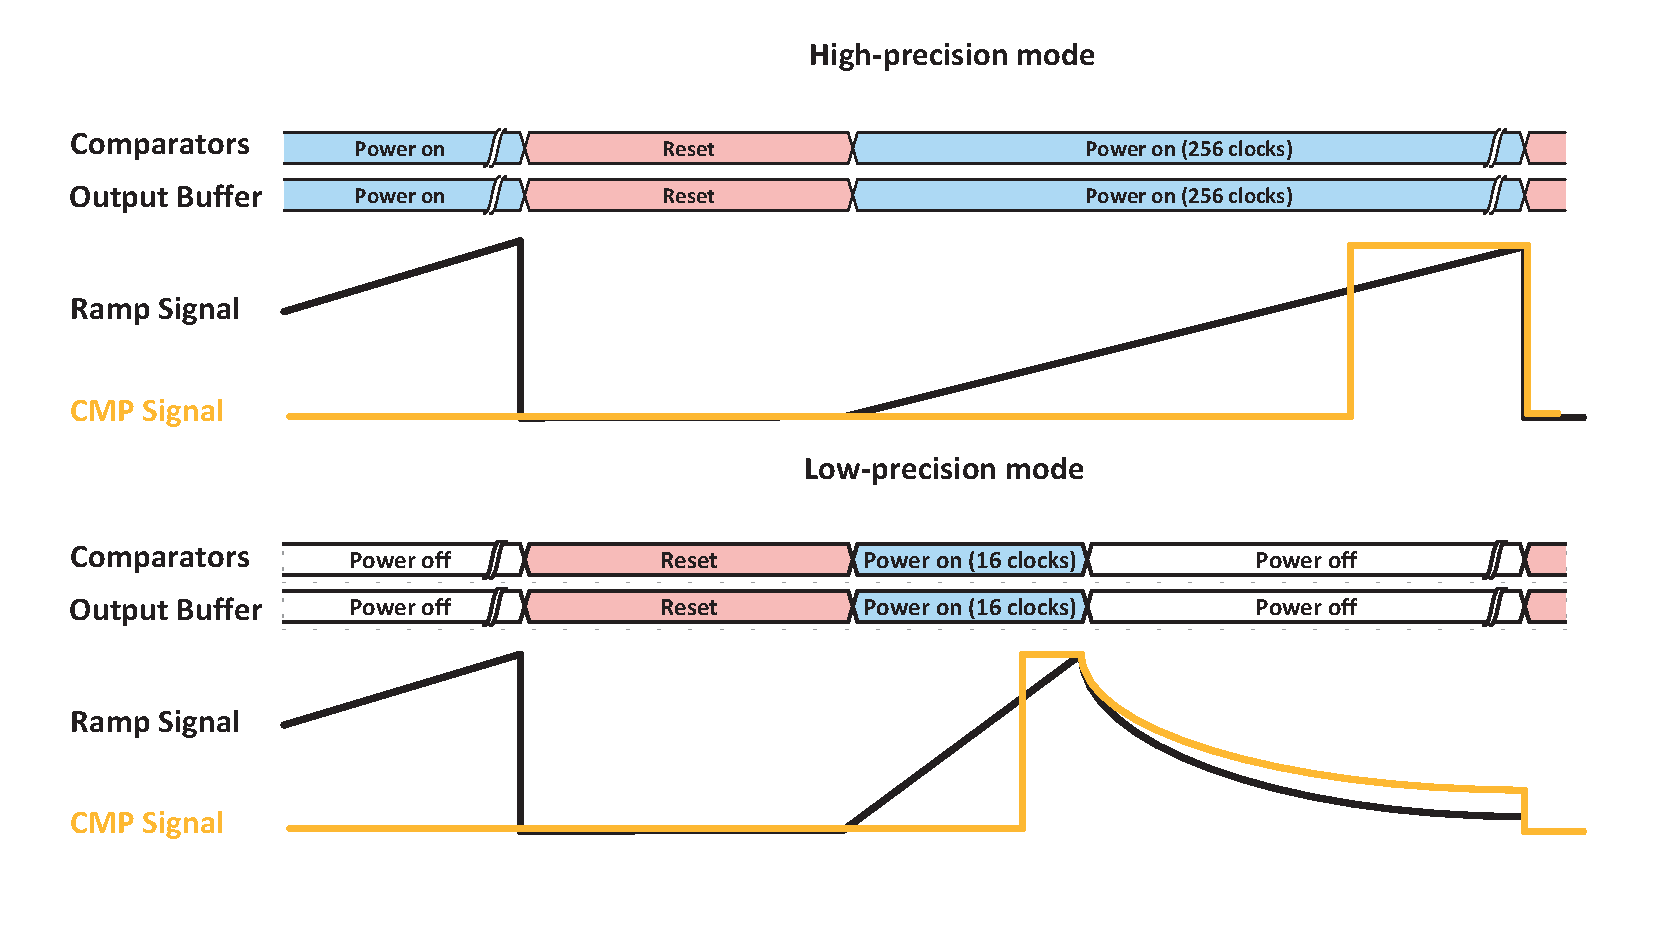
\includegraphics[width=3.5in]{./Figures/SS_pg.eps}}
	\caption{Adaptive-precision and Power Gating Implementation for the SS ADCs.}
	\label{SS_pg}
\end{figure} 

\begin{figure}[htbp]
	\centerline{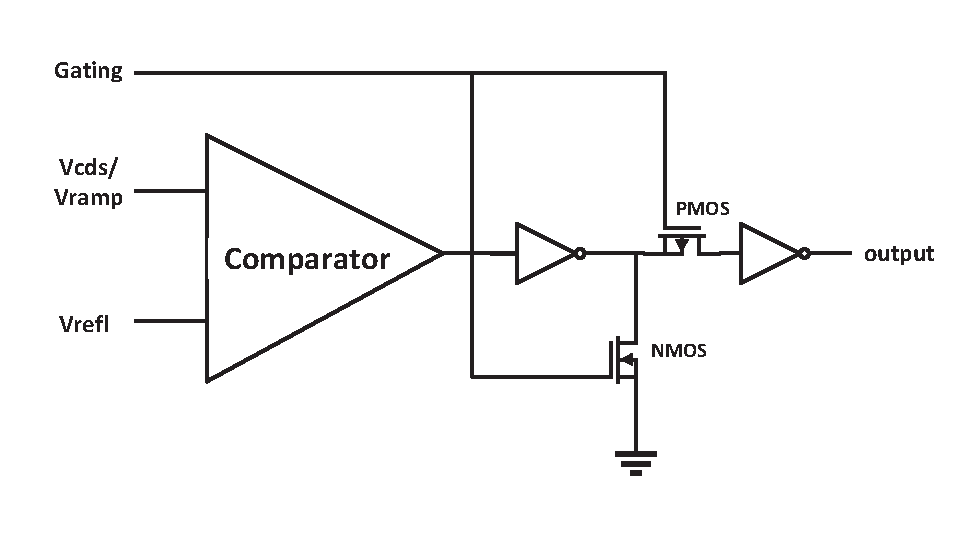
\includegraphics[width=3.5in]{./Figures/MATE.eps}}
	\caption{Two Switches Added to the Inverters Following the Comparator in the SS ADCs.}
	\label{MATE}
\end{figure} 

\subsection{Adaptive-Precision Implementation for the SAR/SS ADCs}

As evaluated in Sect.~\ref{result}, the SAR/SS ADCs’ power consumption is mainly taken up by the column-parallel buffers of reference voltages in the SAR sub-ADCs.
It is because that these buffers need to drive relatively large and changing load capacitance, which means relatively large static and dynamical current is required.
Therefore, gating these buffers will significantly reduce both static power consumption and dynamical power consumption for the ADCs.

In addition, the CDS circuits and comparators in the SAR/SS ADCs also consume a certain amount of energy. However, we only choose to take the comparators under control because they can conveniently share the same gating signal as the buffers'. And the gating signal of the buffers can also be the same as the start signal of the ramp generator. Therefore, gating the buffers and comparators in the SAR/SS ADCs will cost little extra control logic but some shared level-shifters and inverters.

Besides, the power distribution results in Sect.~\ref{result} shows that adaptive-precision tuning is not necessary within the ramp generator of the SAR/SS ADCs, which means the counter in the SAR/SS ADCs do not need to support two modes for adaptive-precision as in the SS ADCs.

The waveform of related signals is presented in Fig.~\ref{SAR_pg}. It is noticed that For low-precison conversion, the ramp signal is generated as usaual but the buffers and comparators will be power off, leaving the 4-bit results converted completely by the SAR logic. 

\begin{figure}[htbp]
	\centerline{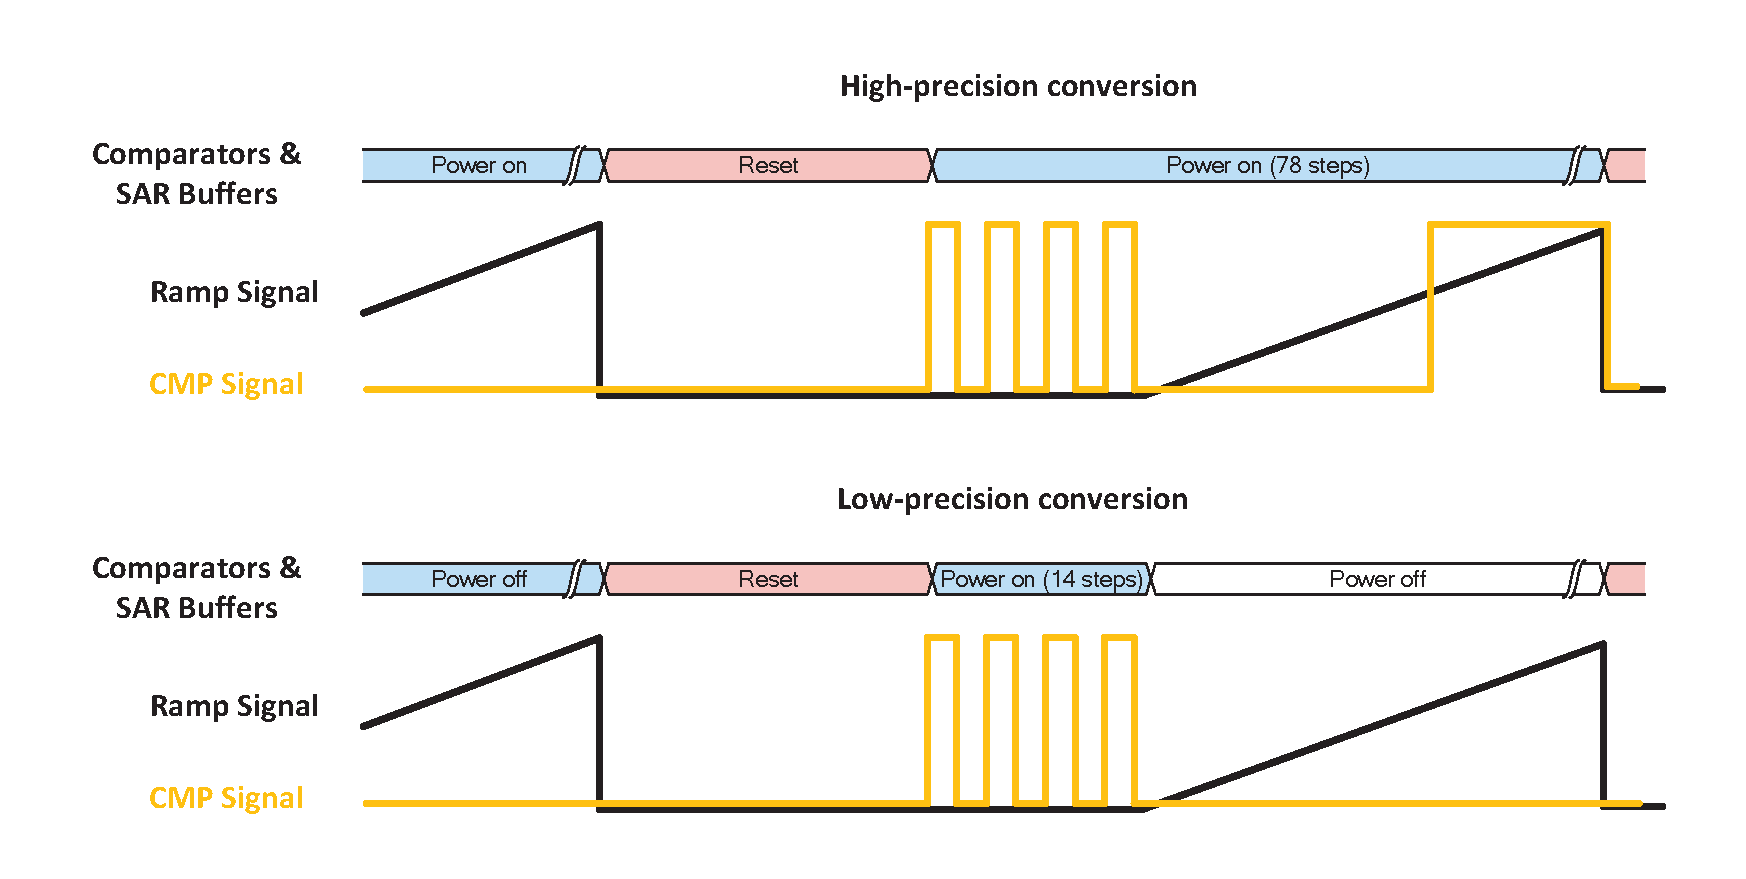
\includegraphics[width=3.5in]{./Figures/SAR_pg.eps}}
	\caption{Adaptive-precision and Power Gating Implementation for the SAR/SS ADCs.}
	\label{SAR_pg}
\end{figure} 